\documentclass{article}

\usepackage[hmargin=.65in, vmargin=.75in]{geometry}
\usepackage[citecolor=blue, colorlinks=True, linkcolor=blue, urlcolor=blue]{hyperref}
\usepackage{natbib}
\usepackage{graphicx}
\usepackage{authblk}
\usepackage[toc,page]{appendix}

\title{A Standard for Exchangeable Magnetotelluric Metadata}
\date{\textbf{Version 0.0.1c -- May 2020}\footnote{\noindent\textbf{\textit{Corresponding Authors:}}
		
		Jared Peacock (\url{jpeacock@usgs.gov})
		
		Andy Frassetto (\url{andy.frassetto@iris.edu})}}
\author[1]{Working Group for Data Handling and Software - PASSCAL Magnetotelluric Program}
\affil[1]{Portable Array Seismic Studies of the Continental Lithosphere, Incorporated Research Institutions for Seismology}

\newcommand{\attr}[1]{\textbf{#1}}
\renewcommand{\arraystretch}{1.25}

\begin{document}
	
\maketitle

\tableofcontents
\vspace{1cm}

\newpage

\section{Introduction}

Researchers using magnetotelluric (MT) methods lack a standardized format for storing time series data and metadata. Commercially available MT instruments produce data in formats that range from proprietary binary to ASCII, and recent datasets from the U.S. MT community have utilized institutional formats or heavily adapted formats like miniSEED. In many cases, the available metadata for these time series are incomplete and only loosely standardized, and overall these datasets are not "user friendly". This lack of resources impedes the exchange and broader use of these data beyond a small community of specialists.

The \href{https://www.iris.edu/hq/programs/passcal/magnetotelluricnstrumentation}{IRIS PASSCAL MT facility} maintains a pool of MT instruments that are freely available to U.S. Principal Investigators (PIs). Datasets collected with these instruments are subject to data sharing requirements, and an IRIS \href{https://www.iris.edu/hq/aboutris/governance/mtoft}{working group} advises the development of sustainable data formats and workflows for this facility. Following in the spirit of the standard created for \href{https://library.seg.org/doi/10.1190/geo2018-0679.1}{MT transfer function} datasets, this document outlines a new metadata standard for MT time series. This standard is a key pillar of MTH5, a new data format which we propose for the international community of MT practitioners. Further information regarding MTH5 will be available later in 2020.

The Python 3 module written for these standards are found at \url{https://github.com/kujaku11/MTarchive/tree/tables}.

\section{General Structure}

The metadata for a full MT dataset are structured to cover details from single channel time series to the full survey. For simplicity each of the different scales of an MT survey and measurements have been categorized starting from largest to smallest (Figure \ref{fig:example}). These categories are: \verb|Survey|, \verb|Station|, \verb|Run|, \verb|DataLogger|, \verb|Electric Channel|, \verb|Magnetic Channel|, and \verb|Auxiliary Channels|. Each of these are described in subsequent sections.  Required keywords are labeled as \verb|True| and suggested keywords are labeled as \verb|False| a user should try to use as much of the suggested metadata as possible for a full description of the data.  

\begin{figure}[htb!]
	\centering
	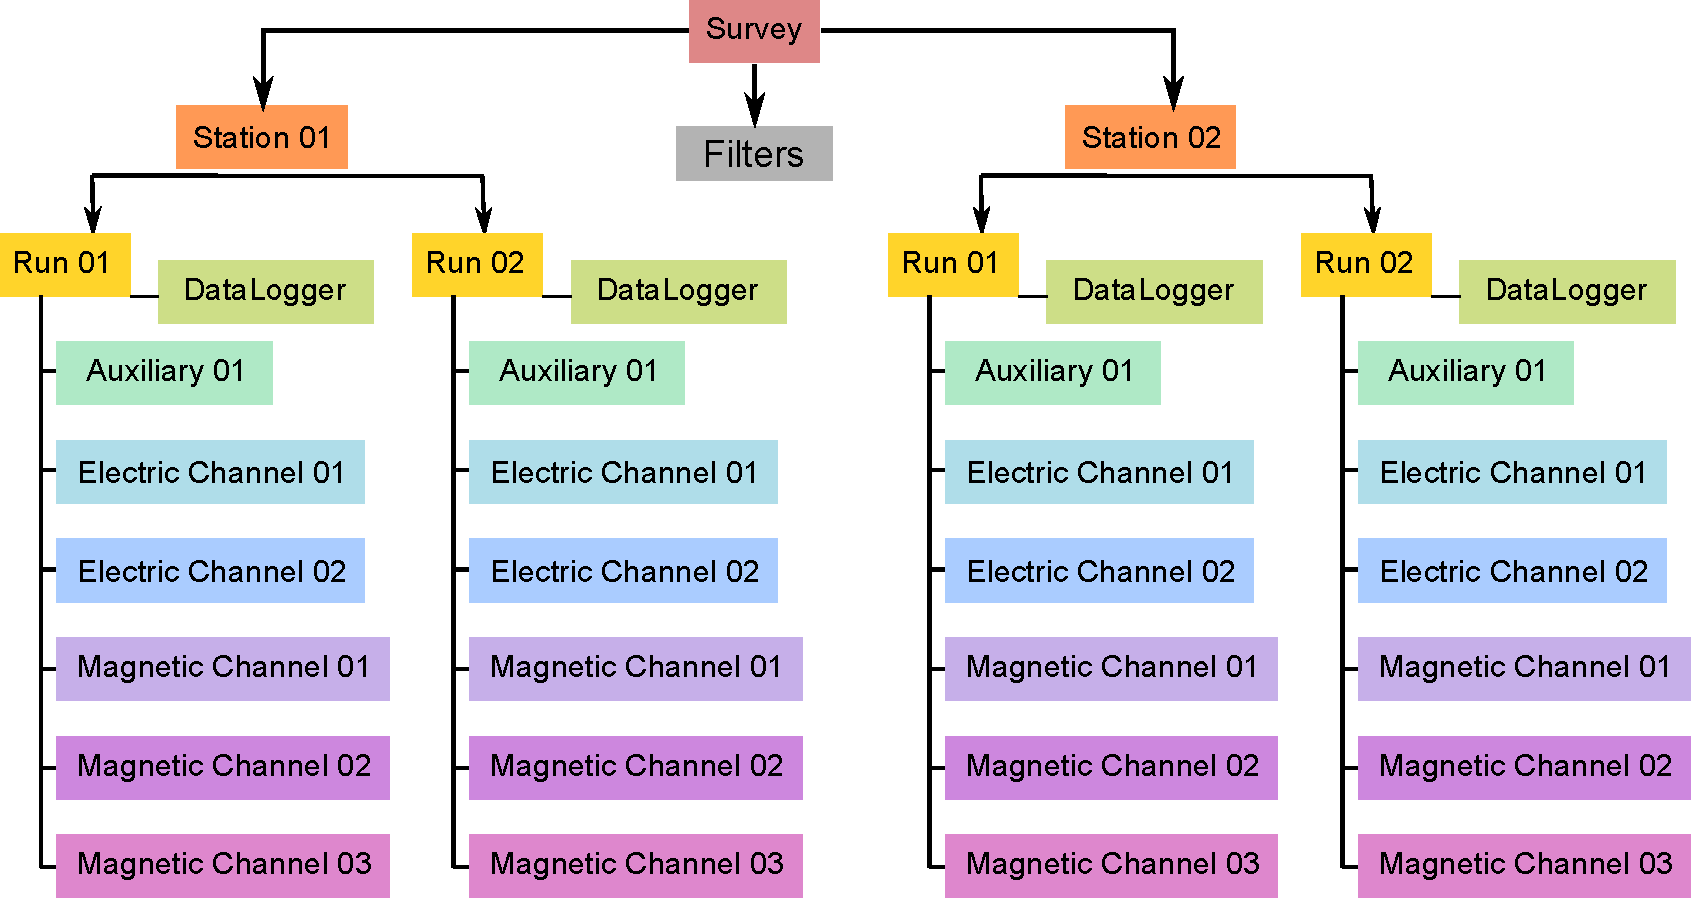
\includegraphics[height=.525\textwidth]{example_mt_file_structure.pdf}
	\caption{Schematic of a MT time series file structure with appropriate metadata. The top level is the \textit{Survey} that contains general information about who, what, when, where, how the data were collected.  Underneath \textit{Survey} are the \textit{Station} and \textit{Filter}.  \textit{Filter} contains information about different filters that need to be applied to the raw data to get appropriate units and calibrated measurements.  Underneath \textit{Station} are \textit{Run} which are blocks where data were collected at a single sampling rate with common start and end time. Finally \textit{Channel} which describes each channel of data collected, this can be an \textit{Auxiliary}, \textit{Electric}, or \textit{Magnetic}.  Metadata is attributed based on the type of data collected in the channel.}
	\label{fig:example}
\end{figure}

\subsection{Metadata Keyword Format}

The metadata key names should be self explanatory and they are structured as follows: \verb|{category}.{name}|, where:
\begin{itemize}
	\item \verb|category| refers to a metadata category that has common parameters, such as \verb|location| which will have a latitude, longitude, and elevation $\longrightarrow$ \verb|location.latitude|, \verb|location.longitude|, and \verb|location.elevation|.  These can be nested, for example \verb|positive.location.latitude|
	\item \verb|name| is a descriptive name, where words should be separated by an underscore. Note that only whole words should be used and abbreviations should be avoided. e.g. \verb|data_quality|.  
\end{itemize}  

As described in this document a '.' represents the separator between different categories.  The metadata can be stored in many different forms.  Common are XML or JSON formats.  See examples below for various ways to represent the metadata.      

\subsection{Formatting Standards}

Specific and required formatting standards for location, time and date, and angles are defined below and should be adhered to.

\subsubsection{Time and Date Format}

All time and dates are given as an ISO formatted date-time string in the UTC time zone.  The ISO date time format is \verb|YYYY-MM-DDThh:mm:ss.ms+00:00|, where UTC is represented by \verb|+00:00|. If the data requires a different time zone this can be accommodated but it is recommended that UTC be used whenever possible. Milliseconds can be accurate to 6 decimal places.  ISO dates are formatted \verb|YYYY-MM-DD|. 

\subsubsection{Location}

All latitude and longitude locations are given in decimal degrees in the well known datum specified at the \verb|Survey| level. \textbf{NOTE: The entire survey should use only one datum that is specified at the Survey level.}

\begin{itemize}
	\setlength\itemsep{0em}
	\item All latitude values must be $<|90|$ and all longitude values must be $<|180|$.
	\item Elevation and other distance values are given in meters.
	\item Datum should be one of the well known datums, WGS84 is preferred, but others are acceptable.
\end{itemize} 

\subsubsection{Angles}

All angles of orientation are given in decimal degrees.  Orientation of channels should be given in geographic coordinates where angles are assumed to be clockwise positive from Geographic North = 0.  If a station was collected not in geographic coordinates this needs to be specified in \verb|station.orientation.option| and the \verb|station.layout_rotation_angle| needs to be specified.   

\subsection{Units}
Units should all be from the metric system.  Abbreviations and full names are acceptable, for example \verb|mV| and \verb|millivolts|.  Table \ref{tab:units} summarizes common acceptable units:


\begin{table}[h!]
	\centering
	\caption[Acceptable units]{Acceptable units}
	\begin{tabular}{|l|c|c|}
		\hline
		\textbf{Measurement Type} & \textbf{Unit Long Name}  & \textbf{Unit Short Name} \\ \hline
		Angles & degrees & deg \\ \hline
		
		Distance &  meters & m \\ \hline
		Latitude/Longitude & decimal degrees & deg \\ \hline
		Resistance & Ohms  &  Ohms \\ \hline
		Resistivity & Ohm-meters & Ohm-m, Ohmm \\ \hline
		Temperature & Celsius & C \\ \hline
		Time & seconds & s \\ \hline
		Voltage & Volts & V \\ \hline
		
		
	\end{tabular}
	\label{tab:units}
\end{table}

\subsection{String Formats}

Each metadata level has a column that describes the style of the input.  These are described in Table \ref{tab:values}.  Note that any list should be comma separated.

\begin{table}[htb!]
	\centering
	\caption[Acceptable String Formats]{Acceptable String Formats}
	\begin{tabular}{|l|p{3.in}|c|}
		\hline
		\textbf{Style} & \textbf{Description}  & \textbf{Example} \\ \hline
		free form & an unregulated string that can contain \{a-z, A-Z, 0-9\} and special characters & This is free form! \\ \hline
		
		alpha numeric & a string that contains no spaces and only characters \{a-z, A-Z, 0-9, -, /, \_\} & WGS84 or GEOMAG-USGS \\ \hline
		controlled vocabulary & Only certain names or words are allowed, in this case examples of acceptable values are provided in the documentation as [ option01 $|$ option02 $|$ ...]. The ... indicates that other options are possible but have not been defined yet. &  station.orientation.option = geographic \\ \hline
		list & list of entries using a comma separator & 'Ex, Ey, Hx, Hy, Hz, T' \\ \hline
		number & a number in the form of the data type, number of decimal places has not been implemented yet & 10.0 for float or 10 for int \\ \hline
		date & ISO formatted date YYYY-MM-DD in UTC & 2020-02-02 \\ \hline
		date time & ISO formatted date time YYYY-MM-DDThh:mm:ss.ms+00:00 in UTC & 2020-02-02T12:20:45.123456+00:00 \\ \hline
		email & a valid email address & \url{person@mt.org} \\ \hline
		url & a full URL that a user could put into a web browser  &  \url{https://www.passcal.nmt.edu/} \\ \hline
		
		
	\end{tabular}
	\label{tab:values}
\end{table}

\clearpage
\newpage
\section{Survey}

A survey describes an entire data set that covers a specific time span and region. This may include multiple PIs in multiple data collection episodes but should be confined to a specific experiment. The \verb|Survey| metadata category describes the general parameters of the survey.

\begin{table}[h!]
	\centering
	\caption[Attributes for Survey]{Attributes for Survey category}
	\begin{tabular}{|l|p{2.75in}|l|c|p{.95in}|}
		\hline
		\textbf{Metadata Key} & \textbf{Description} & \textbf{Type} & \textbf{Required}  & \textbf{Style}  \\ \hline
		acquired\_by.author\ & who acquired the data, this can be different than the project\_lead if a contractor was used & string & True & free form  \\ \hline
		acquired\_by.comments\ & comments about who acquired the data, could include the various groups or contractors & string & False & free form \\ \hline
		archive\_id & alphanumeric name for the project e.g USGS-GEOMAG & string & True & alpha numeric  \\ \hline
		archive\_network & network code given by PASSCAL/IRIS/FDSN & string & True & alpha numeric  \\ \hline
		citation\_dataset.doi & citation dataset doi number & string & True & url  \\ \hline
		citation\_journal.doi & citation journal doi & string & False & url  \\ \hline
		comments\ & comments about survey that are not in the summary & string & False & free form \\ \hline
		country\ & country/countries survey located in, if multiple they should be comma separated & string & False & free form \\ \hline
		datum\ & datum of latitude and longitude coordinates, should be a well-known datum [ WGS84 ] and will be the reference datum for all location & string & True & alpha numeric \\ \hline
		geographic\_name\ & geographic location(s) of survey in general terms & string & True & free form \\ \hline
		name\ & descriptive name of the survey & string & True & free form \\ \hline
		northwest\_corner.latitude\ & location of northwest corner of survey & float & True & number \\ \hline
		northwest\_corner.longitude\ & location of northwest corner of survey & float & True & number \\ \hline
		project & alphanumeric name for the project e.g USGS-GEOMAG & string & True & alpha numeric  \\ \hline
		project\_lead.email & email address of the project lead & string & True & email  \\ \hline
		project\_lead.name & name of the project lead & string & True & free form  \\ \hline
		project\_lead.organization & name of the organization for the project lead & string & True & free form  \\ \hline
		release\_status\ & defined status of how the data can be used. Options are [ Unrestricted Release $|$ Paper Citation Required $|$ Academic Use Only $|$ Conditions Apply ] & string & True & controlled vocabulary \\ \hline
		southeast\_corner.latitude\ & location of southeast corner of survey & float & True & number \\ \hline
		southeast\_corner.longitude\ & location of southeast corner of survey & float & True & number \\ \hline
		summary\ & summary paragraph of survey including the purpose, difficulties, data quality, summary of outcomes if the data have been processed and modeled & string & True & free form \\ \hline
		time\_period.end\_date\ & end date of survey in UTC & string & True & date  \\ \hline
		time\_period.start\_date\ & start date of survey in UTC & string & True & date \\ \hline
	
	\end{tabular}
	\label{tab:survey}
\end{table} 

\newpage
\subsection{Example Survey XML Element}

\begin{verbatim}
<?xml version="1.0" ?>
<survey>
    <acquired_by>
        <author>MT Graduate Students</author>
        <comments>Multiple over 5 years</comments>
    </acquired_by>
    <archive_id>SAM1990</archive_id>
    <archive_network>EM</archive_network>
    <citation_dataset>
        <doi>https://doi.###</doi>
    </citation_dataset>
    <citation_journal>
        <doi>https://doi.###</doi>
    </citation_journal>
    <comments>None</comments>
    <country>USA, Canada</country>
    <datum>WGS84</datum>
    <geographic_name>Yukon</geographic_name>
    <name>Imaging Gold Deposits of the Yukon Province</name>
    <northwest_corner>
        <latitude type="float" units="decimal degrees">-130</latitude>
        <longitude type="float" units="decimal degrees">75.9</longitude>
    </northwest_corner>
    <project>AURORA</project>
    <project_lead>
        <email>m.tee@mt.org</email>
        <organization>EM Ltd.</organization>
        <author>M. Tee</author>
    </project_lead>
    <release_status>Unrestricted Release</release_status>
    <southeast_corner>
        <latitude type="float" units="decimal degrees">-110.0</latitude>
        <longitude type="float" units="decimal degrees">65.12</longitude>
    </southeast_corner>
    <summary>This survey spanned multiple years with graduate students
             collecting the data.  Lots of curious bears and moose,
             some interesting signal from the aurora.  Modeled data
             image large scale crustal features like the 
             "fingers of god" that suggest large mineral deposits.
             Evidence for crustal shortening during the Miocene and 
             multiple plutonic events. </summary>
    <time_period>
        <end_date>1995-01-01</end_date>
        <start_date>2020-01-01</start_date>
    </time_period>
</survey>
\end{verbatim}

\newpage
\section{Station}

A station encompasses a single site where data are collected. If the location changes during a run, then a new station should be created. If the sensors, cables, data logger, battery are replaced during a run but the station remains stations, then this can be recorded in the \verb|Run| metadata but does not require a new station entry.

\begin{table}[ht!]
    \caption[Attributes for Station]{Attributes for Station category}
    \begin{tabular}{|l|p{2.80in}|l|l|p{.95in}|}
        \hline
        \textbf{Metadata Key} & \textbf{Description} & \textbf{Type} & \textbf{Required} & \textbf{Style} \\ \hline
        acquired\_by.author\ & person who acquired the station & string & True & free form  \\ \hline
        acquired\_by.comments\ & comments about who acquired the data, could include the various groups or contractors & string & True & free form \\ \hline
        archive\_id\ & 5 char name \{A-Z; 1-9\} for station & string & True & alpha numeric \\ \hline
        channel\_layout & how the station was laid out. Options [ X $|$ L $|$ ...] & string & True & controlled vocabulary \\ \hline
        channels\_recorded\ & list of channels recorded  e.g. 'Ex, Ey, Hx, Hy' & string & True & list \\ \hline
        comments\ & any comments about station & string & False & free form \\ \hline
        data\_type\ & type of data collected, options: [ BBMT $|$ LPMT $|$ AMT $|$ Combo $|$ ...] see Table \ref{tab:em} & string & True &  controlled vocabulary \\ \hline
        geographic\_name\ & closest geographic reference name to station  & string & True & free form\\ \hline
        id\ & name of the station & string & True & free form\\ \hline
        location.declination.comments\ & comments on the declination & string & True & \\ \hline
        location.declination.model\ & name of the declination model. Options: [ EMAG2 $|$ EMM $|$ HDGM $|$ IGRF $|$ WMM ] see \url{https://www.ngdc.noaa.gov/geomag/} for definitions & string & True & controlled vocabulary \\ \hline
        location.declination.value\ & declination value & float & True & number \\ \hline
        location.latitude\ & longitude location for station & float & True & number \\ \hline
        location.longitude\ & latitude location for station & float & True & number\\ \hline
        location.elevation\ & elevation of station & float & True & number \\ \hline
        orientation.option & orientation coordinate system [ geographic $|$ geomagnetic $|$ channel-measurement specific $|$ ...] & string & True & controlled vocabulary \\ \hline
        orientation.method & method of orienting the channels [ compass $|$ differential GPS $|$ gyroscope $|$...] & string & False & controlled vocabulary \\ \hline
        orientation.layout\_rotation\_angle & if the data were collected in a coordinate system not geographic, this will specify the angle at which all channels were rotated by. & float & False & number \\ \hline
        provenance.creation\_time & creation time of time series data for storing & string & True & date time\\ \hline
        provenance.comments\ & any comments on the history of the data & string & False & free form\\ \hline
        provenance.log\ & log of any changes made to time series data & string & False & free form\\ \hline
        provenance.software.author\ & author of software used to store time series & string & True & free form\\ \hline
        provenance.software.name\ & name of software used to store time series & string & True & free form\\ \hline
        provenance.software.version\ & version of software used to store time series & string & True & free form\\ \hline
        provenance.submitter.author\ & name of person or group archive data & string & True & free form\\ \hline
        provenance.submitter.email\ & email of person or group archiving & string & True  & email \\ \hline
        provenance.submitter.organization\ & name of organization or institution archiving & string & True & free form \\ \hline
        time\_period.start\ & start time and date of data logging in UTC & string & True & date time\\ \hline
        time\_period.end\ & stop time and date of data logging in UTC & string & True & date time \\ \hline
    \end{tabular}
\label{tab:station01}
\end{table}    

\clearpage   
\newpage
\subsection{Example Station JSON}

\begin{verbatim}
{
    "station": {
        "acquired_by": {
            "author": "mt",
            "comments": null
        },
        "archive_id": "MT012",
        "channel_layout": "L",
        "channels_recorded": "Ex, Ey, Hx, Hy",
        "comments": null,
        "data_type": "MT",
        "geographic_name": "Whitehorse",
        "id": "Curious Bears Hallabaloo",
        "location": {
            "latitude": 10.0,
            "longitude": -112.98,
            "elevation": 1234.0,
            "declination": {
                "value": 12.3,
                "comments": null,
                "model": "WMM"
            }
        },
        "orientation": {
            "method": "compass",
            "option": "geographic",
            "layout_rotation_angle": 0.0
        },
        "provenance": {
            "comments": null,
            "creation_time": "1980-01-01T00:00:00+00:00",
            "log": null,
            "software": {
                "author": "test",
                "version": "1.0a",
                "name": "name"
            },
            "submitter": {
                "author": "name",
                "organization": null,
                "email": "test@here.org"
            }
        },
        "time_period": {
            "end": "1980-01-01T00:00:00+00:00",
            "start": "1980-01-01T00:00:00+00:00"
        }
    }
}
\end{verbatim}

\newpage
\section{Run}

A run represents data collected at a single station with a single sampling rate. If the dipole length or other such station parameters are changed between runs, this would require adding a new run.  If the station is relocated then a new station should be created.  If a run has channels that drop out, the start and end period will be the minimum time and maximum time for all channels recorded. 

\begin{table}[h!]
    \caption[Attributes for Run]{Attributes for Run category}
    \begin{tabular}{|l|p{2.55in}|l|l|p{.95in}|}
        \hline
       \textbf{Metadata Key} & \textbf{Description} & \textbf{Type} & \textbf{Required} & \textbf{Style}\\ \hline acquired\_by.author & author name & string & True & free form  \\ \hline
       acquired\_by.comments & email of the contact person & string & False & email  \\ \hline
       channels\_recorded\_auxiliary & list of auxiliary channels recorded & string & True & list  \\ \hline
       channels\_recorded\_electric & list of electric channels recorded. See Table \ref{tab:channel_types} and Table \ref{tab:diretions} & string & True & list  \\ \hline
       channels\_recorded\_magnetic & list of magnetic channels recorded. See Table \ref{tab:channel_types}  and Table \ref{tab:diretions} & string & True & list  \\ \hline
       comments & any comments on the run. See Table \ref{tab:channel_types}  and Table \ref{tab:diretions} & string & False & free form  \\ \hline
       data\_logger.firmware.author & author of the firmware & string & False & free form  \\ \hline
       data\_logger.firmware.name & firmware name & string & False & free form  \\ \hline
       data\_logger.firmware.version & firmware version & string & False & free form  \\ \hline
       data\_logger.id & instrument ID number can be serial number or a designated ID & string & True & free form  \\ \hline
       data\_logger.manufacturer & who manufactured the instrument & string & True & free form  \\ \hline
       data\_logger.model & model version of the instrument & string & False & free form  \\ \hline
       data\_logger.power\_source.comments & any comment about the battery & string & False & free form  \\ \hline
       data\_logger.power\_source.id & battery id & string & False & free form\\ \hline
       data\_logger.power\_source.type & battery type & string & True & free form  \\ \hline
       data\_logger.power\_source.voltage.end & end voltage & float & False & number  \\ \hline
       data\_logger.power\_source.voltage.start & starting voltage & float & False & number  \\ \hline
       data\_logger.timing\_system.comments & any comment on timing system & string & False & free form  \\ \hline
       data\_logger.timing\_system.drift & estimated drift of the timing system & float & False & number  \\ \hline
       data\_logger.timing\_system.type & type of timing system & string & False & free form  \\ \hline
       data\_logger.timing\_system.uncertainty & estimated uncertainty of the timing system & float & False & number  \\ \hline
       data\_logger.type & instrument type & string & True & free form  \\ \hline
       data\_type & type of data recoreded for this run. Options: [ BBMT $|$ LPMT $|$ AMT $|$ Combo $|$ ...] see Table \ref{tab:em} for more details  & string & True & controlled vocabulary  \\ \hline
       id & run ID should be station.archive\_id\{a-z\} & string & True & alpha numeric  \\ \hline
       metadata\_by.author & metadata author name & string & True & free form  \\ \hline
       metadata\_by.comments & comments on metadata & string & False & free form  \\ \hline
       provenance.comments & any comments on provenance of the data & string & False & free form  \\ \hline
       provenance.log & a history of changes made to the data & string & False & free form  \\ \hline
       sampling\_rate & rate of sampling renureded for this run & float & True & number  \\ \hline
       time\_period.end & maximum end time of all run channels & string & True & date time  \\ \hline
       time\_period.start & minimum start time of all run channels & string & True & date time  \\ \hline
    \end{tabular}
    \label{tab:run}
\end{table}

\newpage
\subsection{Example Run XML Element}

\begin{verbatim}
<run>
    <acquired_by>
        <author>T. Lurric</author>
        <email>mt@mt.org</email>
    </acquired_by>
    <channels_recorded_auxiliary>[Temperature]</channels_recorded_auxiliary>
    <channels_recorded_electric>[Ex, Ey]</channels_recorded_electric>
    <channels_recorded_magnetic>[Hx, Hy, Hz]</channels_recorded_magnetic>
    <comments>None</comments>
    <data_logger>
        <id>instrument01</id>
        <manufacturer>MT r' US</manufacturer>
        <type>32 bit digital</type>
        <model>best</model>
        <timing_system>
            <comments>Internal clock locked every 10 seconds</comments>
            <drift type="float" units="seconds">0.00001</drift>
            <type>GPS</type>
            <uncertainty type="float" units="seconds">0.0001</uncertainty>
        </timing_system>
        <firmware>
            <author>T. Lurric</author>
            <version>12.34c</version>
            <name>MTGDC</name>
        </firmware>
        <power_source>
            <type>Pb-acid gel cell</type>
            <id>10</id>
            <voltage>
                <start type="float" units="volts">13.9</start>
                <end type="float" units="volts">12.1</end>
            </voltage>
            <comments>connector cable chewed by rats</comments>
        </power_source>
    </data_logger>
    <data_type>BBMT</data_type>
    <id>mt01a</id>
    <metadata_by>
         <author>student</author>
         <comments>lazy</comments>
    </metadata_by>
    <provenance>
        <comments>redone by grad student</comments>
        <log>2020-01-01T00:00:00+00:00 updated metadata</log>
    </provenance>
    <sampling_rate type="float" units="samples per second">256.0</sampling_rate>
    <time_period>
        <start>2020-01-01T00:00:00+00:00</start>
        <end>2020-02-01T00:00:00+00:00</end>
    </time_period>
</run>
\end{verbatim}

\newpage
\section{Electric Channel}

Electric channel refers to a dipole measurement of the electric field for a single station for a single run.   
 
\begin{table}[h!]
    \caption[Attributes for Electric Channel]{Attributes for Electric category}
    \begin{tabular}{|l|p{2.75in}|l|l|p{.95in}|}
    	\hline
    	\textbf{Metadata Key} & \textbf{Description} & \textbf{Type} & \textbf{Required} & \textbf{Style}\\ \hline
	ac.end & ending AC value; if more than one measurement input as a list of number [1, ...] & float & False & number \\ \hline
	ac.start & starting AC value; if more than one measurement input as a list of number [1, ...] & float & False & number \\ \hline
	channel\_number & channel number on the data logger & integer & True & number \\ \hline
	comments & any comments about the channel & string & False & free form \\ \hline
	component & name of the component measured. Options: [Ex $|$ Ey $|$ Ez $|$ E\# ] & string & True & controlled vocabulary \\ \hline
	contact\_resistance.end & starting contact resistance; if more than one measurement input as a list of number [1, ...] & float & False & number list \\ \hline
	contact\_resistance.start & starting contact resistance; if more than one measurement input as a list of number [1, ...] & float & False & number list \\ \hline
	data\_quality.rating.author & author of who rated the data & string & False & free form \\ \hline
	data\_quality.rating.method & the method used to rate the data & string & False & free form \\ \hline
	data\_quality.rating.value & a rating from 1-5 where 1 is bad and 5 is good and 0 if unrated & integer & True & number \\ \hline
	data\_quality.warning & any warnings about the data that should be noted & string & False & free form \\ \hline
	dc.end & ending DC value; if more than one measurement input as a list of number [1, ...] & float & False & number \\ \hline
	dc.start & starting DC value; if more than one measurement input as a list of number [1, ...] & float & False & number \\ \hline
	dipole\_length & length of the dipole & float & True & number \\ \hline
	filter.applied & boolean if filter has been applied or not. If more than one filter input as a comma separated list.  Needs to be the same length as name or if only one entry is given it is assumed to apply to all filters listed. & boolean & True & list \\ \hline
	filter.comments & any comments on filters & string & False & name \\ \hline
	filter.name & name of filter applied or to be applies. If more than one filter input as a comma separated list & string & True & list \\ \hline
	measurement\_azimuth & azimuth of channel in measurement coordinates & float & True & number \\ \hline
    
    \end{tabular}
    \label{tab:electric01}
\end{table}    

\newpage
\begin{table}[h!]
    \caption[Attributes for Electric Channel cont`d]{Attributes for Electric category continued}
    \begin{tabular}{|l|p{2.75in}|l|l|p{.95in}|}
    	\hline
    	\textbf{Metadata Key} & \textbf{Description} & \textbf{Type} & \textbf{Required} & \textbf{Style}\\ \hline
   		negative.elevation & elevation of location in datum specified at survey level & float & False & number \\ \hline
    	negative.id & instrument ID number can be serial number or a designated ID & string & False & free form \\ \hline
    	negative.latitude & latitude of location in datum specified at survey level & float & False & number \\ \hline
    	negative.longitude & longitude of location in datum specified at survey level & float & False & number \\ \hline
    	negative.manufacturer & who manufactured the instrument & string & False & free form \\ \hline
    	negative.model & model version of the instrument & string & False & free form \\ \hline
    	negative.type & instrument type & string & True & free form \\ \hline
       	positive.elevation & elevation of location in datum specified at survey level & float & False & number \\ \hline
        positive.id & instrument ID number can be serial number or a designated ID & string & False & free form \\ \hline
        positive.latitude & latitude of location in datum specified at survey level & float & False & number \\ \hline
        positive.longitude & longitude of location in datum specified at survey level & float & False & number \\ \hline
        positive.manufacturer & who manufactured the instrument & string & False & free form \\ \hline
        positive.model & model version of the instrument & string & False & free form \\ \hline
        positive.type & instrument type & string & True & free form \\ \hline
        sample\_rate & sample rate & float & True & number \\ \hline
        time\_period.end & end date and time of collection in UTC & string & True & date time \\ \hline
        time\_period.start & start date and time of collection in UTC & string & True & date time \\ \hline
        type & data type for the channel [ electric ]& string & True & controlled vocabulary \\ \hline
        units & units of the data [ counts $|$ V ] & string & True & controlled vocabulary \\ \hline
        \end{tabular}
        \label{tab:electric02}
\end{table}    

\clearpage
\newpage
\subsection{Example Electric Channel JSON}

\begin{verbatim}
{
 "electric": {
    "ac.end": 10.2,
    "ac.start": 12.1,
    "channel_number": 2,
    "comments": null,
    "component": "EX",
    "contact_resistance.end": 1.2,
    "contact_resistance.start": 1.1,
    "data_quality.rating.author": "mt",
    "data_quality.rating.method": "ml",
    "data_quality.rating.value": 4,
    "data_quality.warning": null,
    "dc.end": 1.0,
    "dc.start": 2.0,
    "dipole_length": 100.0,
    "filter.applied": [False],
    "filter.comments": null,
    "filter.name": [ "counts2mv", "lowpass"],
    "measurement_azimuth": 90.0,
    "negative.elevation": 100.0,
    "negative.id": "a",
    "negative.latitude": 12.12,
    "negative.longitude": -111.12,
    "negative.manufacturer": "test",
    "negative.model": "fats",
    "negative.type": "pb-pbcl",
    "positive.elevation": 101.0,
    "positive.id": "b",
    "positive.latitude": 12.123,
    "positive.longitude": -111.14,
    "positive.manufacturer": "test",
    "positive.model": "fats",
    "positive.type": "ag-agcl",
    "sample_rate": 256.0,
    "time_period.end": "1980-01-01T00:00:00+00:00",
    "time_period.start": "2020-01-01T00:00:00+00:00",
    "type": "electric",
    "units": "counts"
  }
}
\end{verbatim}

\clearpage
\newpage
\section{Magnetic Channel}

A magnetic channel is a recording of one component of the magnetic field at a single station for a single run.

\begin{table}[h!]
    \caption[Attributes for Magnetic Channel]{Attributes for Magnetic category}
    \begin{tabular}{|l|p{2.75in}|l|l|p{.95in}|}
    	\hline
    	\textbf{Metadata Key} & \textbf{Description} & \textbf{Type} & \textbf{Required} & \textbf{Style}\\ \hline
   	channel\_number & channel number on the data logger & integer & True & number  \\ \hline	
	comments & any comments about the channel & string & False & free form  \\ \hline
	component & name of the magnetic component measured. Options: [ Hx $|$ Hy $|$ Hz $|$ H\# ] & string & True & controlled vocabulary  \\ \hline
	data\_quality.rating.author & author of who rated the data & string & False & free form  \\ \hline
	data\_quality.rating.method & the method used to rate the data & string & False & free form  \\ \hline
	data\_quality.rating.value & a rating from 1-5 where 1 is bad and 5 is good and 0 if unrated & integer & True & number  \\ \hline
	data\_quality.warning & any warnings about the data that should be noted & string & False & free form  \\ \hline
	filter.applied & boolean if filter has been applied or not. If more than one filter input as a comma separated list.  Needs to be the same length as name or if only one entry is given it is assumed to apply to all filters listed. & boolean & True & list  \\ \hline
	filter.comments & any comments on filters & string & False & name  \\ \hline
	filter.name & name of filter applied or to be applies. If more than one filter input as a comma separated list & string & True & list  \\ \hline
	h\_field\_max.end & maximum magnetic field strength at end & float & False & number  \\ \hline
	h\_field\_max.start & maximum magnetic field strength at beginning & float & False & number  \\ \hline
	h\_field\_min.end & minimum magnetic field strength at end  & float & False & number  \\ \hline
	h\_field\_min.start & minimum magnetic field strength at beginning & float & False & number  \\ \hline
	location.elevation & elevation of location in datum specified at survey level & float & False & number  \\ \hline
	location.latitude & latitude of location in datum specified at survey level & float & False & number  \\ \hline
	location.longitude & longitude of location in datum specified at survey level & float & False & number  \\ \hline
	measurement\_azimuth & azimuth of channel in measurement coordinates & float & True & number  \\ \hline
	sample\_rate & sample rate & float & True & number  \\ \hline
	sensor.id & instrument ID number can be serial number or a designated ID & string & True & free form  \\ \hline
	sensor.manufacturer & who manufactured the instrument & string & True & free form  \\ \hline
	sensor.model & model version of the instrument & string & False & free form  \\ \hline
	sensor.type & instrument type & string & True & free form  \\ \hline
	time\_period.end & end date and time of collection in UTC & string & True & date time  \\ \hline
	time\_period.start & start date and time of collection in UTC & string & True & date time  \\ \hline
	type & data type for the channel & string & True & free form  \\ \hline
	units & units of the data. Options: [counts $|$ nT ] & string & True & controlled vocabulary  \\ \hline
        \end{tabular}
    \label{tab:magnetic}
\end{table}

\newpage
\subsection{Example Magnetic Channel JSON}

\begin{verbatim}
{
    "magnetic": {
        "comments": null,
        "component": "Hz",
        "data_logger": {
            "channel_number": 2
        },
        "data_quality": {
            "warning": "periodic pipeline",
            "rating": {
                "author": "M. Tee",
                "method": "Machine Learning",
                "value": 3
            }
        },
        "filter": {
            "name": ["counts2nT", "lowpass_mag"],
            "applied": [true, false],
            "comments": null
        },
        "h_field_max": {
            "start": 40000.,
            "end": 420000.
        },
        "h_field_min": {
            "start": 38000.,
            "end": 39500.
        },
        "location": {
            "latitude": 25.89,
            "longitude": -110.98,
            "elevation": 1234.5
        },
        "measurement_azimuth": 0.0,
        "sample_rate": 64.0,
        "sensor": {
            "id": 'spud',
            "manufacturer": "F. McAraday",
            "type": "tri-axial fluxgate",
            "model": "top hat"
        },
        "time_period": {
            "end": "2010-01-01T00:00:00+00:00",
            "start": "2020-01-01T00:00:00+00:00"
        },
        "type": "magnetic",
        "units": "nT"
    }
}
\end{verbatim}

\newpage
\section{Filters}

\verb|Filters| is a table that holds information on any filters that need to be applied to get physical units, and filters that were applied to the data to analyze the signal.  This includes calibrations, notch filters, conversion of counts to units, etc. The actual filter will be an array of numbers contained within an array named \verb|name| and formatted according to \verb|type|. The preferred format for a filter is a look-up table which internally can be converted to other formats. 

It is important to note that filters will be identified by name and must be consistent throughout the file. Names should be descriptive and self evident. Examples:
\begin{itemize}
    \item \verb|coil_2284| $\longrightarrow$ induction coil number 2284
    \item \verb|counts2mv| $\longrightarrow$ conversion from counts to mV
    \item \verb|e_gain| $\longrightarrow$ electric field gain 
    \item \verb|datalogger_024| $\longrightarrow$ data logger number 24 response
    \item \verb|notch_60hz| $\longrightarrow$ notch filter for 60 Hz and harmonics
    \item \verb|lowpass_10hz| $\longrightarrow$ low pass filter below 10 Hz
\end{itemize}

In each channel there are keys to identify filters that can or have been applied to the data to get an appropriate signal.  This can be a list of filter names or a single filter name.  An \verb|applied| key also exists for the user to input whether that filter has been applied.  Can be a single Boolean \verb|True| if all filters have been applied, \verb|False| if none of the filters have been applied.  Or can be a list the same length and the filter list identifying if the filter has been applied.  \verb|name: "[counts2mv, notch_60hz, e_gain]"| and \verb|applied: "[True, False, True]"|. 

\begin{table}[htb!]
    \caption[Attributes for Filter]{Attributes for Filters}
    \begin{tabular}{|l|p{2.75in}|l|l|p{.95in}|}
    	\hline
    	\textbf{Metadata Key} & \textbf{Description} & \textbf{Type} & \textbf{Required} & \textbf{Style}\\ \hline
        type\ & type of filter [look up $|$ poles-zeros $|$ converter $|$ FIR $|$ ...]& string &  True  & controlled vocabulary \\ \hline
        name\ & unique name for the filter such that it is easy to query & string & True  & alpha numeric\\ \hline
        units\_in\ & units of data going in [ counts $|$ mV/km $|$ ... ] & string & True  & free form\\ \hline
        units\_out\ & units of data coming out [ counts $|$ mV/km $|$ ... ] & string & True  &  free form \\ \hline
        calibration\_date\ & date of calibration & string &  True  &  date time\\ \hline
        comments\ & any comments on the filtering & string &  False  &  free form \\ \hline
    \end{tabular}
    \label{tab:filter}
\end{table}

\subsection{Example Filter JSON} 

\begin{verbatim}
{
    "filter":{
        "type": "look up",
         "name": "counts2mv",
         "units_in": "counts",
         "units_out": "mV",
         "calibration_date": "2015-07-01",
        "comments": "Accurate to 0.001 mV"
    }
}
\end{verbatim}

\newpage

\section{Auxiliary Channels}

Auxiliary channels include state of health channels, temperature, etc.  

\begin{table}[htb!]
    \caption[Attributes for Auxiliary Channel]{Attributes for Auxiliary category}
    \begin{tabular}{|l|p{2.75in}|l|l|p{.95in}|}
    	\hline
    	\textbf{Metadata Key} & \textbf{Description} & \textbf{Type} & \textbf{Required} & \textbf{Style}\\ \hline
    	channel\_number & channel number on the data logger & integer & True & number  \\ \hline 
    	comments & any comments about the channel & string & False & free form  \\ \hline
        component & name of the component measured. Options [ Temperature $|$ batter\_voltage $|$ state\_of\_health $|$ ...] & string & True & controlled vocabulary  \\ \hline
        data\_quality.rating.author & author of who rated the data & string & False & free form  \\ \hline
        data\_quality.rating.method & the method used to rate the data & string & False & free form  \\ \hline
        data\_quality.rating.value & a rating from 1-5 where 1 is bad and 5 is good and 0 if unrated & integer & True & number  \\ \hline
        data\_quality.warning & any warnings about the data that should be noted & string & False & free form  \\ \hline
        filter.applied & boolean if filter has been applied or not. If more than one filter input as a comma separated list.  Needs to be the same length as name or if only one entry is given it is assumed to apply to all filters listed. & boolean & True & list  \\ \hline
        filter.comments & any comments on filters & string & False & name  \\ \hline
        filter.name & name of filter applied or to be applies. If more than one filter input as a comma separated list & string & True & list  \\ \hline
        location.elevation & elevation of location in datum specified at survey level & float & False & number  \\ \hline
        location.latitude & latitude of location in datum specified at survey level & float & False & number  \\ \hline
        location.longitude & longitude of location in datum specified at survey level & float & False & number  \\ \hline
        measurement\_azimuth & azimuth of channel in measurement coordinates & float & True & number  \\ \hline
        sample\_rate & sample rate & float & True & number  \\ \hline
        time\_period.end & end date and time of collection in UTC & string & True & date time  \\ \hline
        time\_period.start & start date and time of collection in UTC & string & True & date time  \\ \hline
        type & data type for the channel & string & True & free form  \\ \hline
        units & units of the data options are related to the data type [ counts $|$ ... ] & string & True & controlled vocabulary \\ \hline
    \end{tabular}
    \label{tab:aux}
\end{table}

\newpage
\subsection{Example Auxiliary JSON} 

\begin{verbatim}
<auxiliary>
    <comments>great</comments>
    <component>Temperature</component>
    <data_logger>
        <channel_number type="integer">1</channel_number>
    </data_logger>
    <data_quality>
        <warning>None</warning>
        <rating>
            <author>mt</author>
            <method>ml</method>
            <value type="integer">4</value>
        </rating>
    </data_quality>
    <filter>
        <name>
            <i>lowpass</i>
            <i>counts2mv</i>
        </name>
        <applied type="boolean">
            <i type="boolean">True</i>
        </applied>
        <comments>test</comments>
    </filter>
    <location>
        <latitude type="float" units="degrees">12.324</latitude>
        <longitude type="float" units="degrees">-112.03</longitude>
        <elevation type="float" units="degrees">1234.0</elevation>
    </location>
    <measurement_azimuth type="float" units="degrees">0.0</measurement_azimuth>
    <sample_rate type="float" units="samples per second">8.0</sample_rate>
    <time_period>
        <end>2020-01-01T00:00:00+00:00</end>
        <start>2020-01-04T00:00:00+00:00</start>
    </time_period>
    <type>auxiliary</type>
    <units>celsius</units>
</auxiliary>
\end{verbatim}

\newpage
\appendix
\section{Option Definitions}
\label{appendix}

\begin{table}[h!]
	\centering
	\caption[Electromagnetic Period Bands]{Generalized electromagnetic period bands.  Some overlap, use the closest definition.}
	\begin{tabular}{|l|c|c|}
		\hline
		\textbf{Data Type} & \textbf{Definition}  & \textbf{Period Range [s]} \\ \hline
		RMT & radio magnetotellurics &  $10^{-6}$ -- $10^{-4}$\\ \hline	
		AMT &  audio magnetotellurics & $10^{-4}$ -- $10^{0}$ \\ \hline
		BBMT & broadband magnetotellurics & $10^{-1}$ -- $10^{3}$ \\ \hline
		LPMT & long period magnetotellurics  &  $10^{2}$ -- $10^{5}$ \\ \hline
		ULPMT & ultra long period magnetotellurics  &  $10^{5}$ -- $10^{7}$ \\ \hline		
	\end{tabular}
	\label{tab:em}
\end{table}

\begin{table}[h!]
	\centering
	\caption[Channel Components]{These are the common channel components.  More can be added.}
	\begin{tabular}{|l|c|}
		\hline
		\textbf{Channel Type} & \textbf{Definition} \\ \hline
		E & electric field measurement  \\ \hline	
		H & magnetic field measurement \\ \hline
		T & temperature \\ \hline
		Battery & battery   \\ \hline
		SOH & state-of-health channel   \\ \hline		
	\end{tabular}
	\label{tab:channel_types}
\end{table}

\begin{table}[h!]
	\centering
	\caption[Channel Direction]{Channel Direction.  The convention for many MT setups follows the right-hand-rule with X in the northern direction, Y in the eastern direction, and Z positive down.  If the setup has multiple channels in the same direction they can be labeled with a number.  For instance if you measure multiple electric fields Ex01, Ey01, Ex02, Ey02.}
	\begin{tabular}{|l|c|}
		\hline
		\textbf{Direction} & \textbf{Definition} \\ \hline
		x & north direction  \\ \hline	
		y & east direction \\ \hline
		z & vertical direction \\ \hline
		\# \{0--9\} & variable directions   \\ \hline		
	\end{tabular}
	\label{tab:diretions}
\end{table}

\end{document}
